\documentclass{article}
\usepackage{graphicx}
\usepackage{geometry}
\usepackage{bm}
\usepackage{fancyhdr}
\usepackage{minted}
\geometry{a4paper,left=3cm,right=3cm,top=3cm,bottom=3cm}
\usepackage{amsmath}
\pagestyle{plain}
\begin{document}
\section{Perception of Neural Network}
\subsection{Perceptron}
Perceptron is a simple case of neural network. It has 2 layers of neurons, input layer and output layer.
Suppose $x_{1},...,x_{n}$ is input data and $y$ is output.
$$y=f(\sum_{i=1}^{n}w_{i}x_{i}+\theta),$$ where $f$ is a threshold function.
$$ f(x)=\left\{
\begin{aligned}
1,\ \mathrm{if}\ x\geq0 \\
0,\ \mathrm{if}\ x<0
\end{aligned}
\right.
$$
However, we don't often use this function, because it is not continuous and differentiable.
There are some other functions to replace.
$$\mathrm{sigmoid}(x)=\frac{1}{1+\mathrm{e}^{-x}}$$
$$\mathrm{logistic}(x)=\frac{1-\mathrm{e}^{-x}}{1+\mathrm{e}^{-x}}$$
$$\frac{2}{\pi}\mathrm{arctan}(x)$$
$$\mathrm{gaussian}(x)=2\int_{-\infty}^{x}\frac{1}{2\pi}\mathrm{e}^{-\frac{u^{2}}{2}}\ \mathrm{d}u-1$$
\subsection{Neural Network}
In general cases, there are 1 or more than 1 hidden layers. And the input of a layer is the output of the previous one.(Shown on Figure1)
\begin{figure}[!h]
  \centering
  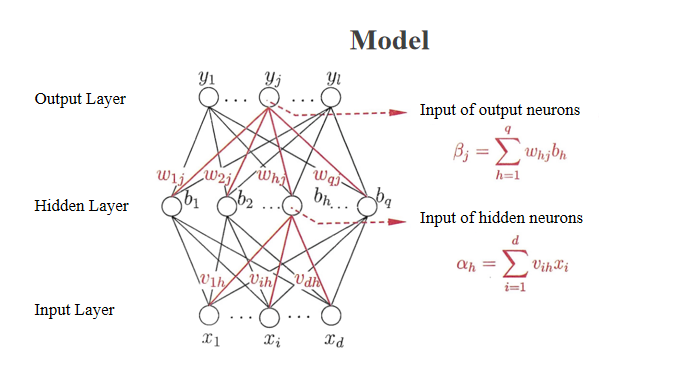
\includegraphics[width=8cm]{1.png}\\
  \caption{Neural Network with 1 Hidden layer}
  \label{}
\end{figure}

And the functional description is$$y_{j}=f(\sum_{k=1}^{q}w_{ij}f(\sum_{s=1}^{d}v_{si}x_{s}+\gamma_{i})+\theta_{j})$$
\subsection{BP Algorithm}
Given a dataset ${(X_{i},Y_{i})}_{i=1,\cdots,n}$, suppose $\widehat{Y}_{i}$ is the output of the neural network with the input $X_{i}$.
We define the error on the sample$(X_{i},Y_{i})$ is$$E_{i}=\frac{1}{2}||\widehat{Y}_{i}-Y_{i}||^{2}$$
And the accumulated error on the dataset is $$E=\frac{1}{m}\sum_{i=1}^{m}E_{i},$$where $m$ is the size of the dataset.

Then, we turn it into an optimization problem. Suppose $\bm{w}$ represents all parameters in neural network model.
$$\bm{w}=\mathop{\arg\min}_{\bm{w}\in W}E$$

In most cases, we use gradient descend method. There are 4 steps.

Step1: Initialize the Connection Weight Randomly from [0,1].

Step2: Input the sample from the train set, and use the output to calculate the error.

Step3: Use the error to renew parameter values in the model, based on gradient descent method.

Step4: Repeat Step2 and Step3, until the error is less than the given error.

But, it is a non-convex optimization problem, which indicates that we may get trapped in local minimum rather than global minimum. Practically we use some
 advanced method such as Simulated Annealing, Stochastic Gradient Descent and Genetic Algorithm.
\subsection{BP Algorithm Demonstration in Python}
\begin{scriptsize}
\begin{minted}{python}
import numpy as np

def sigmoid(x):
    return 1/(1+np.exp(-x))

#standarize the input data
def standardize(In,Out):
    data = np.loadtxt(In)
    m, n = np.size(data, 0), np.size(data, 1)
    for i in range(m):
        for j in range(n):
            data[i][j] = (data[i][j] - data[i].min()) / (data[i].max()-data[i].min())
    np.savetxt(Out, data)

def BPNeutualNetwork(dataset,d,q,l,eta,iteration_number=500):
    D=dataset
    #randomly generate parameters
    theta = np.random.rand(l, 1)
    gamma = np.random.rand(q,1)
    v = np.random.rand(d, q)
    w = np.random.rand(q, l)
    #define intermediate variable
    alpha = np.zeros(q)
    beta = np.zeros(l)
    g = np.zeros(l)
    b = np.zeros(q)
    y_estimate = np.zeros(l)
    #define the error
    E = 0

    for iteration in range(iteration_number):
        E = 0
        for column in range(np.size(D, 1)):
            #get the output
            x = D[:-1, column]
            y = D[-1][column]
            for i in range(np.size(v, 1)):
                alpha[i] = np.array(v[:, i]).dot(x)
            for h in range(np.size(b)):
                b[h]=sigmoid(alpha[h]-gamma[h])
            for i in range(np.size(w, 1)):
                beta[i] = np.array(w[:, i]).dot(b)
            y_estimate = sigmoid(beta - theta)
            #get the error
            E += 0.5 * (y_estimate - y).dot(y_estimate - y)
            #gradient descent method
            g = y_estimate * (1 - y_estimate) * (y - y_estimate)
            w_delta = np.zeros((q, l))
            for i in range(np.size(b)):
                for j in range(np.size(g)):
                    w_delta[i][j] = eta * b[i] * g[j]
            theta_delta = np.zeros(np.size(theta))
            for j in range(np.size(g)):
                theta_delta[j] = -eta * g[j]
            e = np.zeros(np.size(b))
            sumh = np.zeros(np.size(b))
            for h in range(np.size(sumh)):
                for j in range(l):
                    sumh[h] += w[h][j] * g[j]
            e = b * (1 - b) * sumh
            v_delta = np.zeros((d, q))
            for i in range(np.size(x)):
                for h in range(np.size(e)):
                    v_delta[i][h] = eta * e[h] * x[i]
            gamma_delta = np.zeros((q, 1))
            for h in range(np.size(e)):
                gamma_delta[h] = -eta * e[h]
            #renew parameters
            w += w_delta
            theta += theta_delta
            v += v_delta
            gamma += gamma_delta
        #renew the error
        E /= np.size(D, 1)
    #return parameters
    return theta,gamma,v,w,E

#prediction on test set
def calculate(Testdata,v,w,theta,gamma):
    D=Testdata
    alpha = np.zeros(q)
    beta = np.zeros(l)
    b = np.zeros(q)
    y_array=[]
    for column in range(np.size(D, 1)):
        x = D[:-1, column]
        y = D[-1][column]
        for i in range(np.size(v, 1)):
            alpha[i] = np.array(v[:, i]).dot(x)
        for h in range(np.size(b)):
            b[h] = sigmoid(alpha[h] - gamma[h])
        for i in range(np.size(w, 1)):
            beta[i] = np.array(w[:, i]).dot(b)
        y_estimate = sigmoid(beta - theta)
        y_array.append(y_estimate)
    return y_array


if __name__=="__main__":
    standardize('Dataset.txt','DatasetNew.txt')
    d=7       #number of input layer
    q=10      #number of hidden layer
    l=1       #number of output layer
    eta=0.01  #learing rate
    Train = np.loadtxt('Trainingset.txt')
    Test = np.loadtxt('Testset.txt')
    theta,gamma,v,w,E=BPNeutualNetwork(Train,d,q,l,eta,iteration_number=100)
    res=calculate(Test,v,w,theta,gamma)

\end{minted}
\end{scriptsize}
\section{Missing Data}
Suppose sample $\bm{x}$ has $n$ attributes. $\bm{x}=(x_{1},x_{2},...,x_{n})$
And there are $k(k<n)$ attributes missing.

Usually, we have 3 ways to deal with the missing sample.

One way is to delete the sample directly.

The second way is to use the missing data to train the model.

The third way is to fill some value into the missing place. We often use Mean Completer, Hot deck imputation, K-means clustering, Regression and interpolation.
\end{document}
